\section{Llamada del rector} \label{dynProbTilde}
\begin{wrapfigure}{r}{0.3\linewidth}
	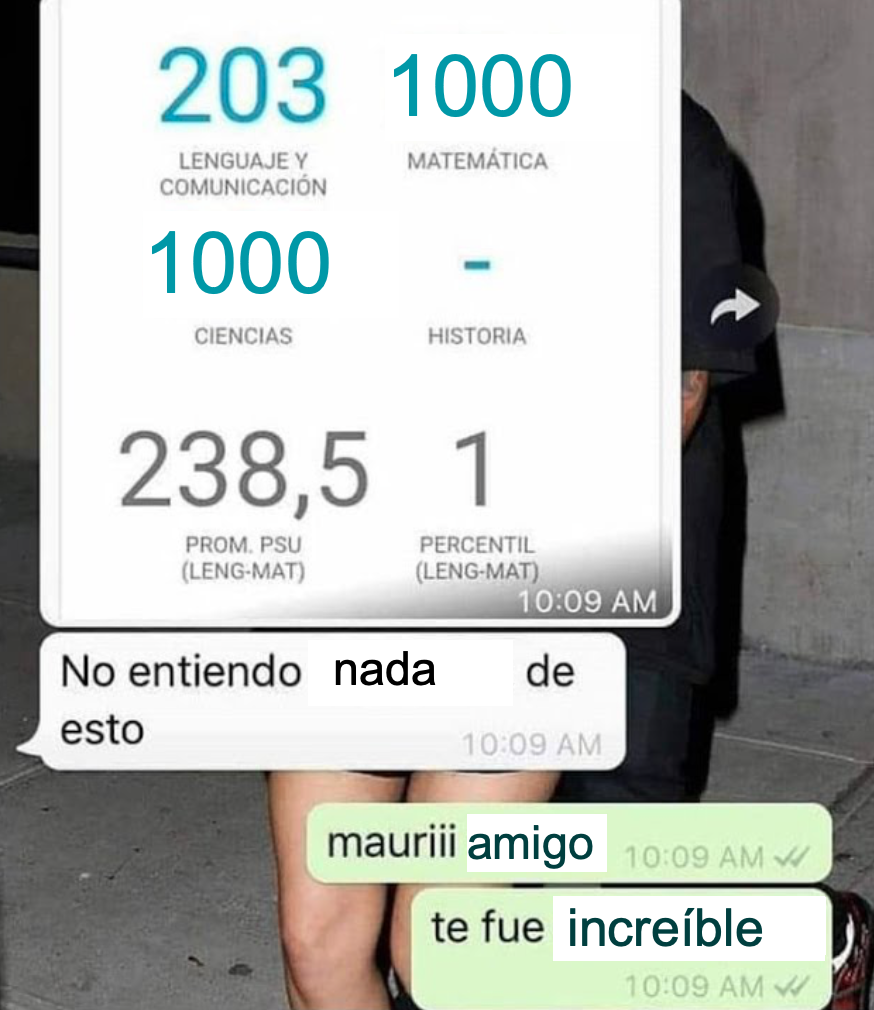
\includegraphics[width=\linewidth]{puntajePAES.png}
	\caption{Deficiencia en lenguaje}
	\label{puntajePAES}
\end{wrapfigure}
Los egresados de la Universidad Técnica Fantástica Suprema de los Mejor (UTFSM) son profesionales increíbles. Destacan en cuanto a sus conocimientos en las ciencias y sus habilidades de resolución de problemas son insupereables. Sólo hay un gran problema: no tienen desarrolladas las habilidades del lenguaje.\\
El rector de la universidad está muy preocupado, y te ha llamado específicamente a tí para que lo ayudes a resolver esta crísis. En esta ocasión tu misión es crear un programa que ayude a mejorar la ortografía de sus alumnos:\\
El alumno usuario del programa deberá introducir una palabra con sus sílabas separadas por un guión `\texttt{-}'. Una de estas será la sílaba tónica, es decir la que contiene al acento prosódico de la palabra; esta estará indicada teniendo su vocal en mayuscula.
El programa deberá verificar si, al seguir las \href{https://lenguaje.com/reglas-de-acentuacion/}{reglas de acentuación} la palabra introducida debiese tener tilde o no. Sólo se deben implementar las reglas fundamentales de las palabras agudas, graves, esdrújulas y sobreesdrújulas.\\

\textbf{INPUT}\\
Cada línea contiene un entero $n$, seguido por $n$ caracteres. Se debe dejar de recibir entradas una vez que $n = 0$\\

\textbf{OUTPUT}\\
Por cada línea de entrada se debe imprimir la palabra introducida anteriormente, sin separación de sílabas y con la sílaba tónica correctamente tildada o no.\\

\textbf{EJEMPLOS}\\
\sampleBoxes
{8 fI-si-ca\\
	9 cam-pe-On\\
	20 au-to-a-na-li-zAr-se\\
	15 rA-pi-da-men-te\\
	19 re-cor-dAn-do-se-lo\\
	0
}
{física\\
	campeón\\
	autoanalizarse\\
	rápidamente\\
	recordándoselo
}
